\documentclass[tikz,border=2pt]{standalone}
\usepackage{amsmath,amssymb}
\usepackage{tikz}
\usetikzlibrary{arrows.meta}

\begin{document}
% |det A| is the area-scaling factor of A: the unit square becomes a parallelogram of area
% |det A|; det A = 0 means the square is flattened.
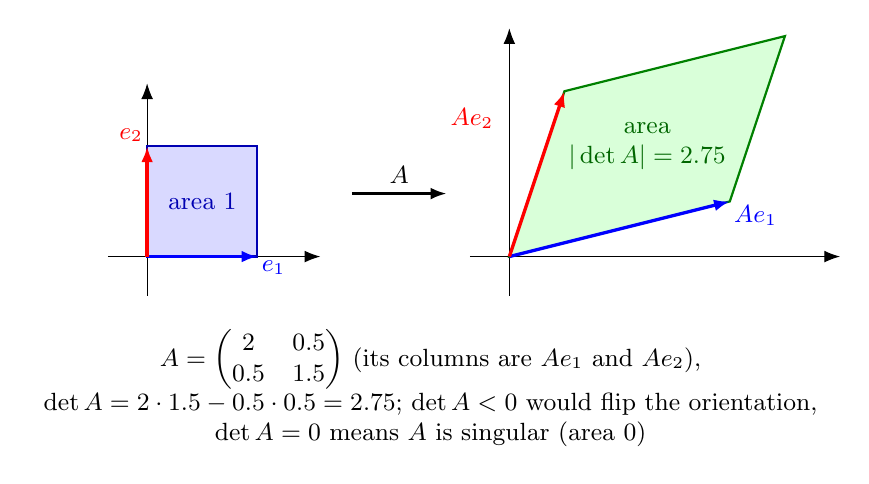
\begin{tikzpicture}[every node/.style={font=\small}, >={Latex[length=2mm]}]
	\draw[->] (-0.5,0) -- (2.2,0);
	\draw[->] (0,-0.5) -- (0,2.2);
	\fill[blue!15] (0,0) rectangle (1.4,1.4);
	\draw[blue!70!black, thick] (0,0) rectangle (1.4,1.4);
	\draw[->, blue, very thick] (0,0) -- (1.4,0) node[below right, inner sep=1pt] {$e_1$};
	\draw[->, red, very thick] (0,0) -- (0,1.4) node[above left, inner sep=1pt] {$e_2$};
	\node[blue!70!black] at (0.7,0.7) {area $1$};
	\draw[->, thick] (2.6,0.8) -- (3.8,0.8) node[midway, above] {$A$};
	\begin{scope}[xshift=4.6cm]
		\draw[->] (-0.5,0) -- (4.2,0);
		\draw[->] (0,-0.5) -- (0,2.9);
		\fill[green!15] (0,0) -- (2.8,0.7) -- (3.5,2.8) -- (0.7,2.1) -- cycle;
		\draw[green!50!black, thick] (0,0) -- (2.8,0.7) -- (3.5,2.8) -- (0.7,2.1) -- cycle;
		\draw[->, blue, very thick] (0,0) -- (2.8,0.7) node[below right, inner sep=1pt] {$Ae_1$};
		\draw[->, red, very thick] (0,0) -- (0.7,2.1);
		\node[red, anchor=east] at (-0.08,1.75) {$Ae_2$};
		\node[green!40!black, font=\small, align=center] at (1.75,1.4) {area\\ $|\det A|=2.75$};
	\end{scope}
	\node[anchor=north, align=flush center, text width=10cm] at (3.6,-0.8) {$A=\begin{pmatrix}2&0.5\\0.5&1.5\end{pmatrix}$ (its columns are $Ae_1$ and $Ae_2$), $\det A=2\cdot1.5-0.5\cdot0.5=2.75$; $\det A<0$ would flip the orientation, $\det A=0$ means $A$ is singular (area $0$)};
\end{tikzpicture}
\end{document}
